\chapter{Ferromagnetismus}
Ferromagnetismus (von lat.: ferrum = Eisen und Magnet) ist die im Alltag am meisten vorkommende Form des Magnetismus, so wie er z.B. in Hufeisen- und Kühlschrankmagneten auftritt. Die Anziehungskraft zwischen einem Magneten und einem ferromagnetischen Material ist verantwortlich für den Großteil der magnetischen Erscheinungen des Alltags.

Ein Material wird "`ferromagnetisch"'  genannt, wenn es in einem externen Magnetfeld selbst magnetisiert wird und diese Magnetisierung auch noch eine Zeit lang beibehält, nachdem das externe Magnetfeld entfernt wurde. Ein solches Material wird von einem Magneten angezogen. Das bekannteste Beispiel hierfür ist Eisen. Die meisten Metalle sind nicht ferromagnetisch und sind daher weder (in ferromagnetischer Weise) magnetisierbar, noch werden sie von einem Magneten angezogen, z.B. Aluminium, Kupfer, Messing, Silber, Gold. Im Alltag lässt sich daher mit einem Magneten leicht prüfen, ob ein metallener Gegenstand aus Eisen ist oder nicht. Eine Ausnahme hiervon stellen austenitische Legierungen dar, die Bestandteil vieler nichtrostender Stähle sind. Ein austenitisches Gefüge ist nicht ferromagnetisch, obwohl es hauptsächlich aus Eisen besteht.
\newline
\section{Vorbereitungsaufgaben}
\begin{itemize}
	\item  Machen Sie sich die Einheiten von B, H, M , $\phi$, $\mu$,  $\mu_0$, $\mu_r$ und j klar.
\newline
\begin{table}[h!]
	\begin{tabular}{lcc}
&& Einheit \\
magnetische Flussdichte&$ [B]$ &1 T = 1$\dfrac{\text{As}}{\text{m}^2}$\\
magnetische Feldstärke&$[H]$ & 1$\dfrac{\text{A} }{\text{m}}$ \\
Magnetisierung&$[M]$ & 1 $\dfrac{\text{A} }{\text{m}}$ \\
magnetischer Fluss&$[\phi]$ &  1 Wb = 1 As  \\
magnetische Feldkonstante&$[\mu_0]$ & $\pi \cdot 10^{-27}\dfrac{\text{N}}{\text{A}^2}$ \\
relative Permeabilität&$[\mu_r]$ & 1 $\dfrac{\text{H}}{\text{M}} = 1 \dfrac{\text{N}}{\text{A}^2}$\\
elektrische Stromdichte&$[j]$ & 1$\dfrac{\text{A}}{\text{m}^2}$

\end{tabular}
\end{table}
%\begin{tabular}{lcr}
%	Han && Einheit && Dimension\\
%	$ [B]$ 1T \\
%	$[H]$ & 2 \\
%	$[M]$ & 2 \\
%	$[\phi]$ & 2 \\
%	$[\mu]$ & 2 \\
%


%[B]
% [H], [M] , $\phi$, $\mu$,  $\mu_0$, $\mu_r$ 
\item 2. Leiten Sie die Beziehung zwischen $\mu$ und $\chi$ her.\\
magnetische Suszeptibilität $\chi$\\
B = $\mu_0(M + H) = \mu_0 \cdot H (\chi + 1) = \mu_0\mu_rH$\\
$\rightarrow$ Permeabilität: $\mu = \chi + 1$

\item 3. Beschreiben Sie die Unterschiede von Diamagnetismus, Paramagnetismus und Ferromagnetismus.
Geben Sie eine mikroskopische Erklärung im Rahmen eines einfachen Atommodells.\\
\underline{Diamagnatismus}: In der Physik werden alle Materialien mit negativer magnetischer Suszeptibilität und ohne magnetische Ordnung als diamagnetisch klassifiziert.
 Diamagnetische Stoffe haben das Bestreben, das Magnetfeld aus ihrem Inneren zu verdrängen. Sie magnetisieren sich gegen die Richtung eines externen Magnetfeldes, folglich ist $\mu_r$ < 1.  \\
 Der Zustand der Teilchen ändert sich bei einer Magnetisierung so, dass ein magnetisches Moment entsteht, das entgegen dem äußeren Magnetfeld entgegenwirkt.\\
\underline{Paramagnetismus}:  In paramagnetischen Stoffen richten sich die atomaren magnetischen Momente in externen Magnetfeldern aus und verstärken damit das Magnetfeld im Inneren des Stoffes. Die Magnetisierung ist also positiv und damit $\mu_r$ > 1.\\
Legt man ein äußeres Magnetfeld an, so werden die mikroskopischen magnetischen Momente ausgerichtet, ohne sich dabei zu beeinflussen. Je stärker das äußere Feld ist, umso paralleler richten sich die magnetischen Momente zum Magnetfeld aus.\\
\underline{Ferromagnetismus}: Ferromagneten richten ihre magnetischen Momente parallel zum äußeren Magnetfeld aus, tun dies aber in einer stark verstärkenden Weise. \\
Unabhängig vom externen Feld besitzt ein Ferromagnet eine spontane Magnetisierung, das externe Feld gibt somit nur die Richtung der Magnetisierung vor.\\
Mikroskopisch gesehen liegt der Unterschied zwischen einem Ferro- und einem Paramagneten darin, dass Ferromagneten eine parallele Ordnung aufweisen, die durch Wechselwirkung unter den einzelnen Momenten auch ohne externes Feld erhalten bleiben.


\item 4. Was sind typische Werte von $\mu_r$ fur magnetische Materialien ?
\newline 
ideal diamagnetischer Leiter: 0\\
Blei/Zinn: 0,999 (diamagnetisch)\\
Platin (paramagnetisch): $1 + 2,6\cdot 10^{-4}$\\
Aluminium (paramagnetisch): 1 + $2,2 \cdot10^{-5}$\\
Eisen (paramagnetisch): 300 bis 10000\\
Kobalt (paramagnetisch): 80 bis 200
\item 5. Sind die Vektoren
$\vec{B}$ und $\vec{H}$ stets parallel? Wie könnte man gegebenenfalls die Nicht-Parallelität
mathematisch ausdrücken?\\
Den magnetischen Fluss kann man durch Erzeugen eines neuen magnetischen Feldes verändern, womit $\vec{B}$ und $\vec{H}$ nicht immer parallel sein müssen. Für ferromagnetische Stoffe gilt, dass $\vec{B}$ und $\vec{H}$ immer parallel sind, nicht aber für diamagnetische Stoffe. Da $\mu_r$ als Tensor darstellbar ist, gilt $\vec{B}$ = $\vec{H}\mu_0\mu_r$ dennoch.
\item 6. Wie groß ist die „differenzielle Permeabilität“ $\partial
B/\partial H$ , wenn die Sättigungsmagnetisierung
erreicht ist?
\newline
Beim Erreichen der Sättigungsmagnetisierung gilt: $\partial B/\partial H$ = 0.
\item 7. Skizzieren Sie qualitativ B(H) und M(H) für ferromagnetische Stoffe. Was ist der Unterschied
zwischen den beiden Graphen?
\newline
\begin{figure}[!h]
	\centering
	\subfigure[Magnetische Flussdichte/Magnetische Feldstärke]	{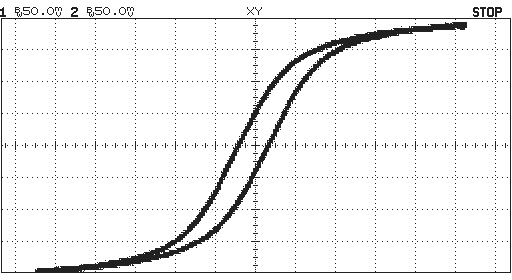
\includegraphics[width=0.45\textwidth]{BHgraph}}
	\hfill
	\subfigure[Magnetisierung/Magnetische Feldstärke; $M_s$=Sättigungsmagnetisierung]{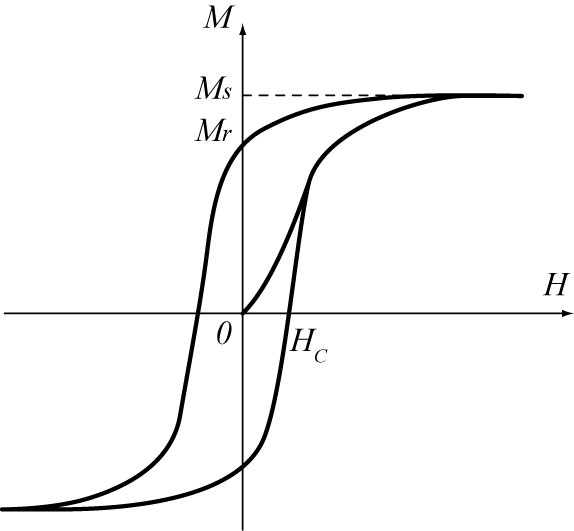
\includegraphics[width=0.45\textwidth]{MHgraph}}

\end{figure}
	Der Unterschied besteht unter Anderem darin, dass die magnetische Flussdichte zum Schluss weiterhin linear ansteigt, während die Magnetisierung nach der Sättigung konstant bleibt.
\item 8. Wie kann man einen ferromagnetischen Körper in einen entmagnetisierten Zustand bringen?
\newline
Einen ferromagnetischen Körper kann man dadurch entmagnetisieren, dass man ihn zum Beispiel erhitzt oder  erschüttert. Auch durch die Wahl eines schnellen Wechselmagnetfeldes und langsames Zurückfahren der Amplituden ist eine Entmagnetisierung möglich.
\item 9. Was ist ein „Querspalt“ und was ein „Längsspalt“? Wozu verwendet man diese?
\newline
Als Längs- bzw. Querspalt werden Hohlräume einer magnetischen Probe bezeichnet, in denen $\vec{H}$ bzw. $\vec{B}$ gemessen werden. Der Querspalt liegt senkrecht zu $\vec{B}$, da sich das B-Feld in dieser Richtung nicht ändert (siehe Maxwellgleichungen). Der Längsspalt liegt wiederum parallel zu $\vec{H}$, da sich so das wirbelfreie H-Feld nicht ändert. \\
\item 10. Warum müssen die Spalte zur Messung von
B und H in ferromagnetischem Material möglichst
eng sein ?
\newline
Die Spalte zur Messung von B und H müssen in ferromagnetischem Material möglichst eng sein, damit die Magnetisierungsverteilung durch die Hohlräume nicht sehr gestört wird.
\item 11. Ist
B in einem nicht-durchgehenden Querspalt genauso groß wie in einem durchgehenden?
\newline
In einem nicht-durchgehenden Querspalt ist B kleiner als in einem durchgehenden, da das Magnetfeld von der "Behinderung", z.B. einem Eisenkern mitgetragen wird.

\item 12. Erklären Sie die Wirkungsweise einer Hallsonde. Was wird mit ihr gemessen? Wie kann man
geometriebedingte Nullfeldsignale vermeiden?
\newline Die Wirkungsweise einer Hall-Sonde beruht auf dem Prinzip des Hall-Effektes und dient der Messung von Magnetfeldern und Strömen.
Man bringt die stromdurchflossene Sonde in ein senkrecht dazu stehendes Magnetfeld und erhält als Ausgangsgröße eine Spannung, die proportional zur magnetischen Feldstärke und zum Strom ist. Auf diese Weise lässt sich bei bekanntem Strom das Magnetfeld ausmessen. Auf der anderen Seite dient die Hall-Sonde auch als Stromstärkemessgerät, wenn das Magnetfeld durch einen stromdurchflossenen Leiter (Spule) erzeugt wird. Hier lässt sich die Stromstärke potentialfrei bestimmen. 
Eine quaderförmige Sonde, meist bestehend aus einem Halbleiter, wird von einem möglichst konstanten elektrischen Strom I in x-Richtung durchflossen. Stromfluss bedeutet hier, dass sich die verfügbare Anzahl freier Elektronen n entgegen der Richtung des extern angelegten elektrischen Feldes mit einer mittleren Geschwindigkeit v bewegt. Die Löcher bewegen sich entsprechend entgegengesetzt. In der bestimmten Zeit t bewegen sich nun alle Ladungsträger, die im Volumen mit der Grundfläche A und einer Höhe h enthalten sind, durch die Grundfläche A hindurch.

Bringt man die Sonde nun in ein magnetisches Feld der Flussdichte B in z-Richtung, so wirkt auf alle orthogonal zum Feld bewegten Ladungen eine Lorentzkraft. Die Ladungen werden an den beiden Seiten der Sonde getrennt. Es entsteht also ein elektrisches Feld in y-Richtung und es wirkt auf die bewegten Ladungen eine Kraft. Kompensiert diese Kraft die Lorentzkraft, sind die Bahnen der bewegten Ladungsträger wieder geradlinig und es kann in y-Richtung die Hallspannung abgegriffen werden.
Die abgegriffene Spannung ist also proportional zur magnetischen Flussdichte. 
Geometriebedingte Nullfeldsignale können mithilfe einer Gegenspannung kompensiert werden.
\item 13. Wozu benutzt man eine „transversale“ bzw. eine „longitudinale Hallsonde“?
\newline
Die transversale Hallsonde wird beim Messen des B-Feldes im Querspalt, die longitudinale beim Messen des H-Feldes im Längsspalt benutzt.
\item 14. Das Magnetfeld einer langen Zylinderspule fällt zu den Spulenden hin ab. Schätzen Sie anschaulich
(ohne zu rechnen!) die Grösse des Feldes an den Spulenenden im Vergleich zur Feldstärke im Mittelpunkt der Spule ab.
\newline
Man stelle sich zwei Spulen nebeneinander vor, die zusammengesetzt eine lange Spule ergeben. Da sich die Feldlinien an den Enden der Einzelspulen an ihren Enden (also in der Mitte von der langen Spule) addieren, ist das Magnetfeld  im Mittelpunkt der Spule etwa doppelt so groß wie an den Spulenenden.
\item 15. Geben Sie die Formel für die magnetische Feldstärke H einer langen Spule als Funktion des Ortes auf der Symmetrieachse an. Stellen Sie diese Abhängigkeit für eine 8cm lange Spule mit Durchmesser D = 5,5cm, Windungszahl n = 500 und Stromstärke I = 2,5A im Intervall +/- 7cm um die Spulenmitte graphisch dar
\newline
$H=\dfrac{NI}{\sqrt{l^2+4r^2}}$\\
$H=\dfrac{NI}{l}\Bigg(\dfrac{l+2x}{2\sqrt{D^2+(l+2x)^2}}+\dfrac{l-2x}{2\sqrt{D^2+(l-2x)^2}}\Bigg)$\\
$H=\dfrac{500\cdot2,5A}{8cm}\Bigg(\dfrac{8cm+2\cdot7cm}{2\sqrt{(5,5cm)^2+(8cm+2\cdot 7cm)^2}}+\dfrac{8cm-2\cdot7cm}{2\sqrt{(5,5cm)^2+(8cm-2\cdot 7cm)^2}}\Bigg)=18,202 \text{A/m}$
\\\\\\\\\\\\\\\\\\\\\\\\\\\\\\

\item 16. Welchen Betrag hat das Erdmagnetfeld in 
Gauss und in Tesla?
\newline Die Stärke und Richtung des Magnetfeldes variieren mit dem Ort der Messung. 
Am Äquator zum Beispiel beträgt das Erdmagnetfeld ca. 30000$\mu T$ = 30$\mu Gs$, am Pol etwa das Doppelte.
%Die horizontale Komponente beträgt in Deutschland etwa $20 \cdot 10^{-6}T = 10^{-2} G$ , die vertikale etwa $44\cdot10^{-6} T = 44\cdot 10^{-2} $. 
\item 17. Wo werden ferromagnetische Stoffe bzw. der Ferromagnetismus von Stoffen in der Praxis genutzt?
\newline
Ferromagnetische Stoffe bzw. Ferromagnetismus werden z.b. in Elektromagneten, Transformatoren oder elektrischen Speichermedien benutzt. Oft ist hierbei die magnetische Sättigung des Kerns unerwünscht und führt zu einem Abfall des Wirkungsgrades. Um eben diese Sättigung zu verhindern, müssen magnetische Kerne in Transformatoren und Elektromotoren eine Mindestquerschnittsfläche aufweisen. In der Geophysik wird Ferromagnetismus zur Identifizierung von Materialien benutzt. 
\end{itemize}

\section{Durchführung}

Zur Durchführung der Versuche stehen Ihnen folgende Geräte zur Verfügung:
\begin{itemize}
	\item Feldmessgerät PHYWE mit transversaler Hallsonde
	\item Feldmessgerät PHYWE mit longitudinaler Hallsonde
	\item div. Experimentiertrafos mit Kernen
	\item Netzgeräte
	\item Multimeter
	\item div. Stativmaterial
\end{itemize}

Achtung! Bitte gehen Sie sehr sorgsam mit den Hallsonden um, sie dürfen keinesfalls
verbogen oder geknickt werden!
Vor dem Umbau des Eisenkerns bitte den Strom am Netzgerät auf Null zurückdrehen,
dann erst ausschalten!
Hallsonde entfernen und in die Stativklemmen einspannen!

\subsection{Aufgabenstellungen}
\underline{Test der Hallsonden mit Hilfe des Erdmagnetfelds}\\
Ermitteln Sie die Richtung des Erdmagnetfelds im Raum mit einer Kompassnadel. Testen Sie die
Hallsonden durch Messung des Erdmagnetfelds und stellen Sie dabei den Nullpunkt korrekt ein. Hal
ten Sie dazu die Hallsonden a) senkrecht, b) parallel und c) antiparallel zum Erdmagnetfeld. Achten
Sie darauf, dass sich keine Eisenteile in unmittelbarer Nähe befinden.
\\\\
\underline{Magnetfeld einer Luftspule}\\
Ermitteln Sie die magnetische Feldstärke H einer Luftspule (Länge l = 7,2cm, Durchmesser D = 5,5cm, Windungszahl n =500), durch die ein konstanter Strom fließt (I =2,5A), auf der Symmetrieachse in Abhängigkeit von der Position (in einem Intervall von +/-7cm um die Spulenmitte). Verwenden Sie dazu die longitudinale Hallsonde. Tragen Sie die Messdaten auf mm-Papier auf. Vergleichen
Sie den gemessenen Verlauf der Feldstärke graphisch mit der für eine Zylinderspule endlicher Länge
bzw. für einen magnetischen Punktdipol theoretisch erwarteten Abhängigkeit.
\\\\
\underline{Magnetfeld einer Spule mit geradem Eisenkern}\\
Setzen Sie nun einen geraden Eisenkern mit Langsbohrung und einem angespitzten Ende in die Spule
ein und führen Sie die gleichen Messungen durch wie bei Aufgabe fm.5.2. Tragen Sie die Messpunkte
in den Graphen von Aufgabe fm.5.2 ein (im gleichen Maßstab, um quantitativ vergleichen zu konnen).
Diskutieren Sie die Veränderung im Feldstärkeverlauf durch Einführung des Eisenkerns mit Hilfe
des Hintergrundwissens aus Kap. fm.2.5 Können Sie daraus auf die relative Permeabilität
$mu_r$ r des
Eisenkerns folgern?
\\\\
\underline{Magnetischer Kreis mit schmalem Luftspalt}\\
Bauen Sie einen magnetischen Kreis mit zwei Spulen à 500 Windungen, einem U-Kern und zwei angespitzten durchbohrten Polschuhen auf (lL = 4mm Luftspalt zwischen den flachen Enden der Polschuhe) (vgl. Abb. fm.4).
Achten Sie auf die Polung der Spulen (die Felder der Einzelspulen sollen sich gegenseitig verstärken
anstatt sich zu kompensieren !) Schliesst man die Spulen besser in Reihe oder parallel ans Netzgerät
an? Messen Sie die magnetische Feldstärke H bei fester Stromstärke (I = 2,5A in jeder der beiden Spu
len) als Funktion des Ortes in der Längsbohrung und einige cm ausserhalb der Bohrung. Achten Sie
auf die Vorzeichen der von den Feldmessgeräten angezeigten Werten! Tragen Sie die Messwerte gra
phisch auf.
Diskutieren Sie den gemessenen Verlauf des Feldes längs der Bohrung. Denken Sie dabei an nicht
vernachlässigbare Streufelder. Versuchen Sie gegebenenfalls unerwartete Ergebnisse zu interpretie
ren.\\

\underline{Ermittlung der Hysteresekurve eines Eisenkerns von Hand}\\
Messen Sie die magnetische Feldstärke H und die magnetische Flussdichte B in Abhängigkeit vom
Spulenstrom I für einen vollen Ummagnetisierungszyklus, ausgehend von der Sättigung. Platzieren
Sie dazu die Hallsonden so, dass die Messung am wenigsten durch Streufelder verfälscht wird.
Um möglichst weit in die Sättigung zu kommen, können Sie kurzzeitig Spulenströme bis zu 5A
zulassen. Achten Sie unbedingt darauf, dass Sie den Strom nur monoton ändern (warum?). Tragen Sie die Messwerte in ein B(H)-Diagramm ein.

